\chapter{Výsledky}

\section{Testovanie}
Pri testovaní vizualizácie sme postupovali podľa článku od Elmqvist et al. \cite{Patterns}, ktorý opisuje najpoužívanejšie vzory testovania vizualizácie a článok od Vogel et al., v ktorom autori testujú webovú vizualizáciu \cite{WebBasedUserTest}.

\subsection{Testovacia procedúra}
Testovanie prebiehalo prostredníctvom niekoľkých úloh, ktoré sme navrhli na základe špecifikácie požiadaviek na vizualizáciu uvedených v sekcii \ref{sec:spec}. 

Každému subjektu bola predstavená základná funkcionalita systému v krátkom 15 minútovom návode. Následne subjekt obdržal testovací formulár (pozri prílohu \ref{sec:testform}) obsahujúci 7 rôznych úloh, ktoré mal subjekt vykonať a po vykonaní každej z nich do formulára zapísať výsledok svojho skúmania.

Pri testovaní sme jednak vyhodnocovali správnosť odpovedí ale aj rýchlosť vykonania jednotlivých úloh. Taktiež sme dokumentovali interakciu s vizualizáciou počas vykonávania úlohy pomocou \textit{screen capture}.

\subsection{Výsledky testovania}

Vizualizáciu sme testovali na 6 subjektoch bez vyššieho meteorologického, matematického alebo informatického vzdelania. Taktiež žiaden užívateľ nemal skúsenosti s verifikáciou predpovedí a náš systém videl prvýkrát v živote. Všetky tieto faktory vplývali na výsledok nášho testu, keďže sme sa často stretali s nepochopením respektíve s pomalým pochopením zadania a teda čas riešenia úlohy sa značne natiahol.

V tabuľke \ref{table:results} môžme vidieť, že všetci testovaní užívatelia vyriešili všetky úlohy správne a výsledky riešenia sa líšili iba v nameranom čase. V tabuľke je hrubým písmom zvýraznený najdlhší a najkratší priemerný čas pre dané úlohy. 
V priemere každá úloha trvala asi pol minúty (26s) a všetky úlohy užívatelia vykonali v priemere za 3 minúty.


\begin{table}[h]
\centering
\caption{Výsledky testovania}
\label{table:results}
\begin{tabular}{|c|c|c|c|}
\hline
\rowcolor[HTML]{9B9B9B} \textbf{Úloha} & \textbf{Počet správnych} & \textbf{Počet nesprávnych} & \textbf{Priemerný čas} \\ \hline
1              &            6             &             0              &         23.85s                       \\ \hline
2              &            6             &             0              &         37.27s                      \\ \hline
3              &            6             &             0              &         24.66s                      \\ \hline
4              &            6             &             0              &         \textbf{40.36}s                      \\ \hline
5              &            6             &             0              &         24.69s                      \\ \hline
6              &            6             &             0              &         \textbf{9.73}s                      \\ \hline
7              &            6             &             0              &         23.27s                       \\ \hline
\rowcolor[HTML]{C0C0C0} \textbf{Suma}  &           \textbf{42}             &             \textbf{0}              &        \textbf{183.83}                      \\ \hline
\end{tabular}
\end{table}

V grafe na obrázku \ref{fig:results} môžme lepšie vidieť sumárne porovnanie časov pre jednotlivé úlohy a užívateľov. Môžme si ľahko všimnúť, že úlohy 1, 2, 5 a 7 majú približne rovnaký priemerný čas, zatiaľ čo úlohy 2, 4 mali výrazne dlhšie trvanie a úloha 9 trvala v priemere najkratšie.

Dlhé trvanie úlohy 2 prisudzujeme vyššej zložitosti úlohy oproti ostatným. Pre užívateľov bolo odhalenie outlierov pomerne rýchle, avšak väčšinu času zabralo užívateľom odčítanie z grafu o akú presnú hodnotu a predpoveď ide.

Pri úlohe 4 bolo problémom rýchle odčítanie z grafu, o aký dátum sa jedná. Dôvodom bolo nedobré označenie dátumov na \mbox{$ x $-ovej} škále, kedy sa jednotlivé dni v roku označujú číslami 0-364. Užívateľ uvidel konkrétny dátum, až keď nadišiel myšou na dané miesto, kedy sa mu presné hodnoty ukázali v \textit{tooltipe}. Lepším riešením by bola redšia škála s mesačnými intervalmi alebo konkrétnymi dátumami.

Výsledky nášho testovania považujeme celkovo za uspokojivé, keďže aj neskúsení užívatelia dosahovali pri všetkých úlohách dobré časy. Taktiež nám tieto výsledky poukázali na slabiny našej práce, ktorými sú hlavne zlé alebo slabé označenia škál, grafov a legiend.

\begin{figure}
	\centering
	\includegraphics[width = 5in]{resultchart}
	\caption{Výsledky testovania.}
	\label{fig:results} 
\end{figure}

\section{Demonštrácia}
V tejto časti chceme demonštrovať príklad analýzy fungovania predpovedného modelu pomocou nami navrhnutých techník vizualizácie. Rovnako ako pri testovaní vizualizácie aj tu sme použili predpovedané dáta z modelu WRF. Konkrétne sa jednalo o tlak pri povrchu zeme v hektopaskaloch.

\subsection{Štatistiky}
Na obrázku \ref{fig:overview}a môžme vidieť farebnú mapu (Prehľad) zobrazujúcu RMSE pre celý rok 2012. Ako už vieme zo sekcie \ref{sec:errormeasurement}, RMSE nadobúda iba kladné hodnoty a teda nehovorí nič o smeru chyby, ale iba o jej veľkosti. 

Z daného obrázka ľahko vyčítať niektoré zaujímavé vzory. Ku príkladu je veľmi dobre vidno, že model predpovedá najlepšie v okolí šiestej hodiny predpovede a v okolí poludnia zaznamenávame prudký pokles presnosti predpovedí. Fakt, že model predpovedá najlepšie až okolo šiestej hodiny a nie ihneď na začiatku predpovede trocha nabúra náš predpoklad, že smerom do budúcnosti sa predpoveď zhoršuje. Tu sa potvrdzuje dôležitosť vizualizácie, ktorá slúži nie len na to, aby sme \textit{zistili očakávané}, ale aj \textit{objavili neočakávané}.

Na obrázku \ref{fig:overview}b máme zobrazenú priemernú chybu (MFE), ktorá sa počítala z rovnakých dát ako RMSE na obrázku \ref{fig:overview}a. Na tomto grafe je ihneď vidieť to, či model podhodnocuje alebo nadhodnocuje predpovede. Ako vidíme väčšina grafu je zafarbená na modro, čo značí záporné hodnoty, a teda podhodnotenie predpovedí. Taktiež vďaka dobre zvolenej farebnej škále môžme vidieť, že niektoré hodnoty (napríklad 6 hodina v Januári) sú kladné, avšak stále blízko nuly.

\begin{figure}
	\centering
	\includegraphics[width = 5in]{overview}
	\caption{a) Farebná mapa zobrazujúca RMSE b) Farebná mapa zobrazujúca MFE}
	\label{fig:overview} 
\end{figure}

V prípade, že užívateľ potrebuje získať informáciu o veľkosti a aj smere chyby súčasne, po kliknutí na konkrétny mesiac sa mu zobrazia všetky vypočítané štatistiky súčasne (pozri obrázok \ref{fig:detail}). O aké štatistika sa jedná vidíme v \textit{tooltipe} podľa farebného rozlíšenia.

\begin{figure}
	\centering
	\includegraphics[width = 6.5in]{detail}
	\caption{Zobrazenie RMSE, MFE, MAE a SD (Standard Deviation) na jednom grafe súčasne}
	\label{fig:detail} 
\end{figure}


\subsection{Chyby}

Súčasťou obrazovky vizualizácie je aj zobrazenie jednotlivých chýb, z ktorých sa počítali štatistiky, či už pomocou farebnej mapy alebo pomocou grafov pre vizualizáciu distribúcie chyby.

Farebná mapa na obrázku \ref{fig:errors} nám dáva dobrý obraz o chybách v chronologicky zoradených predpovediach pre mesiac Február. Na tomto grafe si ľahko môžme všimnúť predpovede, ktoré sa nejakým spôsobom odlišujú od ostatných. Napríklad väčšina predpovedí podhodnocuje, ale predpoveď ABC vo väčšine nadhodnocuje, čo môže byť zapríčinené rôznymi vplyvmi. Taktiež si môžme všimnúť, že predpoveď ABC v okoli Xtej hodiny má výrazný výkyv hodnôt a naopak predpoveď ABC v okolí Ytej hodiny výrazne podhodnocuje.


\begin{figure}
	\centering
	\includegraphics[width = 6.5in]{errors}
	\caption{}
	\label{fig:errors} 
\end{figure}

Odporúčame tento typ vizualizácie kombinovať s grafom distribúcie, ako je napríklad na obrázku \ref{fig:XYZ}.


  

